\documentclass[conference]{IEEEtran}

\usepackage{cite}
\usepackage{amsmath,amssymb,amsfonts}
\usepackage{graphicx}
\usepackage{textcomp}
\usepackage{xcolor}
\usepackage{algpseudocode}
\usepackage{algorithm}
\usepackage{cmap}
\usepackage[T1]{fontenc}
\usepackage{lmodern}
\usepackage[french]{babel}
\usepackage{tikz}
\usepackage[hidelinks]{hyperref}
\usetikzlibrary{positioning,fit,arrows.meta,calc}
\usepackage[caption=false,font=footnotesize]{subfig}


\def\BibTeX{{\rm B\kern-.05em{\sc i\kern-.025em b}\kern-.08em
    T\kern-.1667em\lower.7ex\hbox{E}\kern-.125emX}}
    

\begin{document}

\title{BLAST : Basic Local Alignment Search Tool}

\author{\IEEEauthorblockN{Amory ANTAO}
\IEEEauthorblockA{\textit{Université Paris-Cité, M2BI}}\\
\href{mailto:amoryantao@net-c.com}{amoryantao@net-c.com}}

\maketitle

\begin{abstract}
La croissance explosive des données de séquences impose des méthodes rapides et suffisamment sensibles pour détecter des similarités localement pertinentes.\\
Nous réimplémentons BLAST (version originale, ungapped) et gapped BLAST (double-hit et extension gappée avec $x\_drop$) et comparons leurs comportements sur des jeux de tests contrôlés.\\
Les expériences confirment les tendances des articles fondateurs : (i) l’heuristique double-hit réduit fortement le nombre de candidats à étendre, au prix d’un abaissement du seuil de d'acceptance pour créer la liste de mots initiaux, sur les séquences d'acides aminés,  pour conserver la sensibilité ; (ii) à sensibilité comparable, gapped BLAST diminue grandement le temps total d’exécution en limitant les extensions, tout en améliorant la robustesse des alignements grâce aux gaps ; (iii) lorsque le seuil d’acceptation augmente, BLAST I voit rapidement chuter le nombre d’alignements retenus tandis que BLAST II en préserve une fraction plus importante et de meilleure qualité.\\
Globalement, nos résultats reproduisent qualitativement le compromis rapidité/sensibilité de gapped BLAST et valident l’intérêt pratique du double-hit couplé à une extension gappée.
\end{abstract}


\section{Introduction}
github : https://github.com/AntaoA/projet-blast
\subsection{Motivation}
Avec les progrès techniques et technologiques, tous les domaines de la bioinformatique sont confrontés à une croissance constante de la quantité de données disponibles.\\
Cette expansion permet d’accroître considérablement nos connaissances, mais elle exige également des efforts continus pour améliorer l’efficacité des méthodes capables de traiter ces volumes massifs.\\
Parmi les problématiques majeures, la recherche de similarités entre séquences occupe une place centrale : identifier une séquence d’ADN ou de protéine dans une base de données constitue souvent une première étape essentielle pour comprendre et classifier, sur le plan fonctionnel comme sur le plan évolutif, un gène nouvellement séquencé.\\
Les relations évolutives et fonctionnelles se manifestent fréquemment par la conservation de régions locales spécifiques, dont la détection est cruciale pour l’interprétation biologique. Cependant, les approches exactes de comparaison de séquences sont devenues impraticables face à l’explosion de la taille des bases.\\
L’enjeu est donc de concevoir des méthodes capables d’analyser efficacement des ensembles de données gigantesques, tout en conservant une sensibilité suffisante pour détecter des similitudes significatives.\
C’est dans cette perspective que des algorithmes heuristiques, parmi lesquels BLAST est sans doute le plus emblématique, ont été développés et sont aujourd’hui devenus des outils incontournables de la bioinformatique.
\subsection{Contexte}
De très nombreuses méthodes exactes d’alignement de séquences ont été proposées. La plupart reposent sur le paradigme de la programmation dynamique. Parmi elles, on peut citer l’algorithme de Needleman–Wunsch, destiné aux alignements globaux, ou encore celui de Smith–Waterman, qui permet de réaliser des alignements locaux.\\
Ces approches garantissent toujours de trouver une solution optimale au problème posé. Toutefois, cette optimalité a un prix : leur complexité en temps et en mémoire rend leur utilisation difficile dès que la taille des données augmente, ou lorsqu’il est nécessaire de répéter un très grand nombre de comparaisons.\\
Pour surmonter ces limitations, plusieurs chercheurs se sont tournés vers des heuristiques, dans le but de réduire considérablement les temps de calcul. Ces méthodes ne visent pas à fournir une solution strictement optimale, mais cherchent à maintenir une sensibilité suffisante pour obtenir dans la plupart des cas un résultat biologiquement pertinent.\\
Parmi ces approches, FASTP a été l’une des pionnières, mais elle restait limitée en vitesse comme en sensibilité.\\
C’est dans ce contexte que Stephen F. Altschul, Warren Gish, Webb Miller, Eugene W. Myers et David J. Lipman ont proposé en 1990 le Basic Local Alignment Search Tool (BLAST). Cet algorithme, rapidement enrichi par de nombreuses variantes et améliorations, s’est imposé comme une référence incontournable en bioinformatique, et demeure aujourd’hui encore l’un des outils les plus utilisés pour l’alignement de séquences.
\subsection{Objectifs}
L’objectif principal de BLAST était de proposer un algorithme offrant un compromis optimal entre efficacité de calcul et sensibilité biologique.\\
Ce qui a rendu cet outil incontournable n’est pas seulement sa rapidité, mais également sa grande simplicité d’utilisation et la diversité de ses variantes, qui le rendent applicable à différents types de données.\\
Dans le cadre de ce projet, nous nous concentrons sur deux versions majeures de l’algorithme. La première correspond à la version originale décrite en 1990, permettant de réaliser des alignements locaux sur l’ADN comme sur les protéines. La seconde est issue des travaux de 1997, qui introduisent gapped BLAST. Cette variante s’avère plus pertinente d’un point de vue biologique, car elle permet d’intégrer des insertions et des suppressions dans les alignements, phénomène extrêmement fréquent dans l’évolution des séquences.\\
En combinant vitesse et prise en compte des gaps, gapped BLAST constitue une amélioration substantielle par rapport à la version initiale.\\
Après avoir implémenté ces algorithmes, nous comparerons leurs performances aux résultats présentés dans les articles fondateurs, afin d’évaluer la reproductibilité des expériences originales et la fidélité de notre réimplémentation.

\section{Méthodes}

\subsection{BLAST : principes généraux}
BLAST est un algorithme heuristique conçu pour accélérer la recherche d’alignements locaux significatifs.\\
Son principe repose sur la détection, dans une base de données, de courts segments identiques ou fortement similaires à ceux de la séquence requête (appelé query).\\
Ces segments servent de points d’ancrage à partir desquels l’algorithme procède à des extensions locales afin de construire des alignements pertinents.\\
De manière générale, BLAST se décompose en trois étapes principales :
\begin{itemize}
\item Étape 1 : Construction d’une liste de mots à partir de la query, éventuellement enrichie par des voisins
\item Étape 2 : Balayage de la base de données pour repérer les occurrences de ces mots et identifier des positions candidates
\item Étape 3 : Extension des candidats afin de sélectionner uniquement les meilleurs alignements.
\end{itemize}
\subsection{BLAST I}

\subsubsection{ADN}

\paragraph{Construction des mots}
On choisit un paramètre $w$ (en pratique, une valeur typique est $w = 13$ pour l’ADN) et l’on extrait de la query l’ensemble des mots de longueur $w$.\\
Chaque mot est ensuite associé à sa ou ses positions dans la séquence, de manière à constituer un dictionnaire qui servira de point d’entrée pour la recherche de candidats dans la base de données.

\paragraph{Recherche des hits}
Pour chaque séquence de la base de données, une fenêtre de longueur $w$ est glissée le long de la séquence afin d’extraire les segments présents dans notre liste de mots.\\
Les correspondances obtenues sont enregistrées (on parle de hits) et considérées comme candidats à traiter lors de l’étape d’extension.

\paragraph{Extension}
Chaque hit est étendu indépendamment vers la droite puis vers la gauche via de la programmation dynamique.\\
Les seules opérations considérées sont les correspondances exactes (\emph{match}) et les substitutions (\emph{mismatch}).\\
Pour cette étape, nous utilisons une matrice de substitution simple attribuant un score de +5 pour un match et de –4 pour un mismatch.\\
Pour augmenter l'efficacité, on ne réalise pas la programmation dynamique complète. En effet, elle est limitée via un paramètre $x\_drop$ (valeur typique, $x\_drop = 20$).\
Concrètement, le processus d’extension est interrompu dès que le score courant devient inférieur à $score\_max - x\_drop$, ce qui permet d’élaguer rapidement les alignements peu prometteurs.\\
À l’issue de l’extension à gauche et à droite, les résultats sont combinés pour déterminer l’alignement final.\\
On retourne alors les positions, dans la requête et dans la séquence de la base, correspondant au meilleur score obtenu.\\
On utilise un dernier paramètre $S$ (par exemple $S = 80$) nous permettant de retourner uniquement les alignements significatifs (dépassant ce seuil).

\subsubsection{Protéines}

\paragraph{Construction des mots et génération de voisins}
Dans le cas des protéines, l’alphabet des acides aminés étant beaucoup plus vaste que celui de l’ADN, la taille des mots $w$ est réduite afin de maintenir une probabilité raisonnable de détection (en pratique, $w = 3$ est un choix courant).\\
Par ailleurs, la liste des mots extraits de la requête est enrichie par l’ajout de voisins à haut score.\\
Concrètement, pour chaque segment de taille $w$ de la requête, on tente de remplacer chaque acide aminé par une autre lettre de l’alphabet.\\
Si le score associé à ce nouveau mot, calculé à l’aide d’une matrice de substitution (typiquement PAM250 ou BLOSUM62), dépasse un seuil $T$, ce mot voisin est ajouté à la liste.\\
Ce procédé permet d’augmenter la sensibilité de l’algorithme en tenant compte de similarités plausibles issues de substitutions fréquentes dans l’évolution des protéines.

\paragraph{Recherche des hits et extension}
La recherche des hits et leur extension s’effectue de manière identique pour les protéines et pour l’ADN.



\subsection{BLAST II (gapped)}

\subsubsection{Motivation}
La version initiale de BLAST se limite, comme on l’a vu, aux opérations de correspondance exacte match et de substitution.\\
En particulier, elle n’autorise pas les deux autres opérations classiques définies par la distance de Levenshtein : l’insertion et la suppression.\\
Cette restriction permettait déjà de détecter de nombreuses similitudes locales, mais elle restait en décalage avec la réalité biologique.\\
En effet, les alignements pertinents entre protéines ou entre séquences génomiques comportent très fréquemment des gaps, qui résultent de mutations ponctuelles ou d’événements évolutifs.\\
Par conséquent, la sensibilité de la première version de BLAST n’était pas optimale.\\
Par ailleurs, du point de vue de l’efficacité, l’étape la plus coûteuse de BLAST correspond à l’extension des hits, qui représente plus de 90\% du temps total d’exécution. Réduire le nombre de candidats à étendre constitue donc un objectif essentiel pour améliorer les performances.\\
Pour répondre à ces deux problèmes, une évolution majeure a été introduite en 1997 avec le gapped BLAST.\\
Cette version repose sur deux améliorations complémentaires :
\begin{itemize}
\item l’utilisation de double-hits, qui réduit fortement le nombre de candidats retenus pour l’extension
\item l’implémentation d’une extension gappée, autorisant insertions et suppressions, afin de mieux refléter les alignements biologiques réels.
\end{itemize}
De plus, dans l'article original, et dans mon implémentation, on va se limiter au cas des protéines, qui est le plus pertinent biologiquement, même s'il est possible de l'adapter à l'ADN.
\subsubsection{Construction des mots et génération de voisins}
Cette étape est identique à celle décrite pour les protéines dans la version initiale de BLAST.

\subsubsection{Détection de double-hits}
Un second niveau de filtrage est introduit afin de réduire le nombre de candidats à étendre.\\
Seuls les cas où deux hits ne se chevauchant pas, apparaissant sur la même diagonale et étant séparés d’une distance inférieure ou égale à un paramètre $A$ (typiquement $A = 40$) sont retenus.\\
La diagonale correspond à la valeur $x_1 - x_2$, où $x_1$ désigne la position du hit dans la requête et $x_2$ sa position dans la séquence de la base.\\
Intuitivement, deux hits sont situés sur la même diagonale lorsque l’écart entre leurs positions est identique dans la requête et dans la base, c’est-à-dire lorsque le nombre de caractères intermédiaires est le même des deux côtés.\\
Grâce à ce filtrage, seule une petite fraction des hits initiaux est conservée pour l’extension.\\
Afin de maintenir une sensibilité comparable à celle de la version classique, il est nécessaire d’abaisser le seuil d’acceptation des mots voisins $T$ (par exemple $T = 11$).\\
L’implémentation repose sur une table associant à chaque diagonale le dernier hit rencontré.\\
Cela permet, dès l’arrivée d’un nouveau hit, de vérifier immédiatement s’il se chevauche avec le précédent ou s’il respecte la contrainte de distance, et ainsi de décider de sa conservation ou non.

\subsubsection{Extension ungapped et sélection de la graine}
Pour chaque double-hit, une extension ungapped initiale est réalisée autour du second hit afin de calculer un premier score.\\
Si le score obtenu dépasse un seuil $S_g$ (typiquement $S_g = 42$, l’alignement est considéré comme suffisamment prometteur pour déclencher une extension gappée. \\
Dans ce cas on recherche, dans la région détectée, la fenêtre de longueur fixe (typiquement de 11 acides aminés) donnant le meilleur score, et on choisit son centre comme graine pour l’alignement gappé.

\subsubsection{Extension gappée}
L’extension gappée repose également sur la programmation dynamique, mais doit cette fois gérer, en plus des correspondances (match) et substitutions (mismatch), l’introduction de gaps dans la query comme dans la séquence de la base de données.\\
Pour cela, l’implémentation adopte une variante de l’algorithme de Gotoh, adaptée au contexte de BLAST.\\
Deux ajustements principaux sont apportés :
\begin{itemize}
\item une initialisation spécifique, qui contraint l’alignement à débuter par la paire correspondant à la graine retenue (match ou substitution) ;
\item l’utilisation d’un paramètre $x_drop$, comme pour l’extension ungapped, permettant d’interrompre l’exploration lorsque le score est inférieur à $score\_max - x\_drop$.
\end{itemize}
Les coûts associés aux gaps suivent un modèle affine : une pénalité d’ouverture de gap et une pénalité d’extension (typiquement fixées respectivement à $10$ et $1$).\\
Cette combinaison permet à la fois de représenter fidèlement les insertions et suppressions biologiques, et de limiter efficacement le nombre de calculs en élaguant les alignements peu prometteurs.\\
Les résultats sont ensuite combinés pour déterminer l’alignement final, en retenant uniquement ceux dont le score dépasse un seuil $S$ (par exemple $S = 80$), comme pour les extensions ungapped.

\section{Résultats}
\subsection{Nombres de hits}

La Figure~\ref{fig:test_T} illustre l’évolution du nombre de hits simples et doubles en fonction du seuil $T$, pour BLAST I et BLAST II.\\
On observe une décroissance régulière du nombre de hits simples (BLAST I) lorsque $T$ augmente, avec une réduction d’un facteur supérieur à $10$ entre les bornes testées. Les hits doubles (BLAST II) suivent la même tendance mais de manière beaucoup plus marquée : leur nombre diminue d’un facteur proche de $40$ sur le même intervalle.\\
Le décalage de $T$ de $+3$ (simulation BLAST II) nous permet de voir que, pour une sensibilité équivalente, BLAST II trouve $3$ à $5$ fois plus de hits simples, mais seulement seulement $10$ à $20\%$ de hits doubles comparé à BLAST I, ce qui va réduire grandement la phase d'extension.\\
En résumé, ces résultats confirment que l’heuristique à double hit de BLAST II permet de filtrer efficacement le bruit : on réduit le nombre d’extensions déclenchées tout en conservant une sensibilité comparable à BLAST I grâce au réglage adapté du seuil $T$.

\begin{figure}
    \centering
    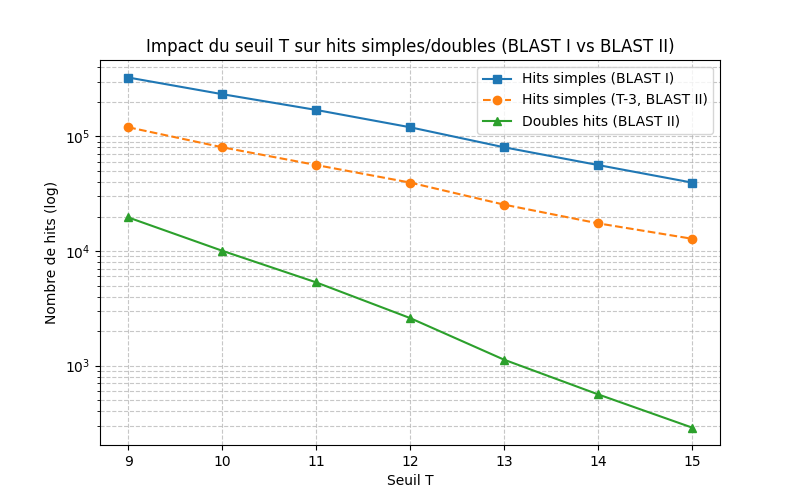
\includegraphics[width=\linewidth]{test_T.png}
    \caption{Nombre de hits simples et doubles en fonction du seuil $T$ pour BLAST I et BLAST II.}
    \label{fig:test_T}
\end{figure}


\subsection{Nombres d'alignements acceptés}

La Figure~\ref{fig:nb_alignments} illustre la différence de comportement entre BLAST I et BLAST II lorsque l’on fait varier le seuil $S_{accept}$.

\paragraph*{Paramètres utilisés.}
BLAST I a été paramétré avec un seuil de mots $T=13$ et une extension non gappée avec un $x\_drop$ de 16, selon les recommandation de l'article original.\\
Pour BLAST~II, on a abaissé le seuil ($T=11$) afin de compenser le critère plus strict de double-hit (fenêtre $A=30$).\\
Les alignements gappés sont déclenchés lorsque le score d’un HSP dépasse $S_{g}=42$, puis étendus avec un $X$-drop gappé plus tolérant ($X_{g}\approx 40$), chose que l'on peut faire puisque l'on a beaucoup moins de candidats.

\paragraph*{Analyse des résultats.}
Pour des valeurs faibles de $S_{accept}$, BLAST I retient un très grand nombre d’alignements, souvent de courte taille et de faible qualité.\\
BLAST II, au contraire, filtre fortement à ce stade : l’exigence de deux hits sur la même diagonale réduit grandement le bruit et ne laisse passer qu’un sous-ensemble d’alignements plus robustes.\\
Lorsque le seuil $S_{accept}$ augmente, on observe un renversement de tendance.\\
Les alignements produits par BLAST I chutent rapidement : les résultats faibles sont éliminés.\\
En revanche, BLAST II conserve une proportion plus importante d’alignements de haute qualité. Ceci s’explique par l’utilisation d’un $X$-drop gappé plus large qui permet de prolonger les alignements malgré la présence de mismatches ou de petites insertions ou suppression, ce qui augmente la probabilité de capter des alignements biologiquement pertinents. 

\paragraph*{Conclusion.}
BLAST I est donc plus sensible mais génère beaucoup de bruit initialement, tandis que BLAST II, grâce au double-hit et à l’extension gappée avec un $x\_drop$ adapté, produit moins d’alignements au départ mais s’avère plus robuste et efficace pour détecter les alignements significatifs lorsque l’on impose des seuils plus stricts.


\begin{figure}
    \centering
    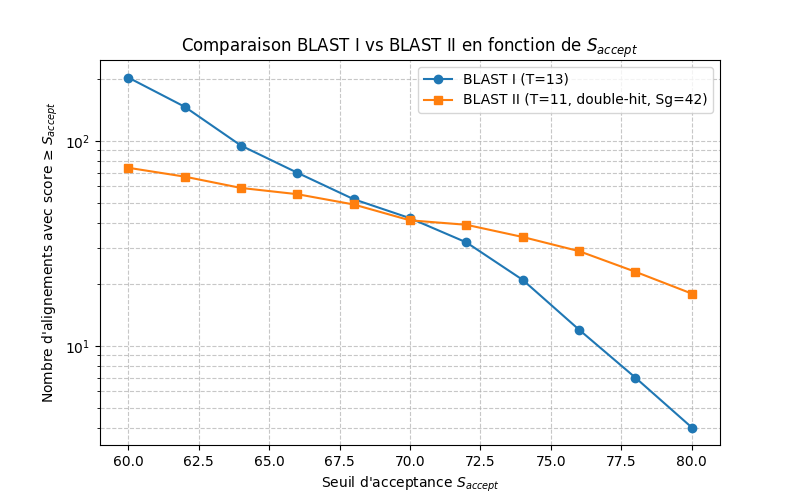
\includegraphics[width=\linewidth]{test_nb_alignments.png}
    \caption{Nombre d'alignements acceptés en fonction du seuil $S_{accept}$ pour BLAST I et BLAST II.}
    \label{fig:nb_alignments}
\end{figure}

\subsection{Vitesse}

La Figure~\ref{fig:time_vs_dbsize} compare les temps d’exécution de BLAST~I (algorithme original, ungapped) et de BLAST~II (avec extension gappée et heuristique du double-hit).\\
Les paramètres ont été choisis pour une sensibilité comparable ($w=3$, BLAST~I avec $T=13$, BLAST~II avec $T=11$, $A=40$, $S_g=42$, $X_{drop}=20$ pour les extensions non gappées et $X_{drop}=40$ pour les extensions gappées).\\

\paragraph*{Répartition du temps par étape.}
Les chronométrages détaillés confirment les observations des articles fondateurs:
\begin{itemize}
    \item Pour BLAST~I, environ $90\%$ du temps total est consacré à l’extension des hits. La grande majorité des 10% restant est utilisé pour trouver les hits dans la base de données.
    \item Pour BLAST~II, la répartition un peu plus équilibrée : les extensions restent toujours majoritaires ($\approx 60-70\%$), mais la phase de recherche de double-hits représente maintenant $30-40\%$ du temps. L’étape de génération de la liste de voisins reste négligeable ($\ll 1\%$).
\end{itemize}

\paragraph*{Analyse comparative.}
On observe que gapped BLAST est $3$ à $4$ fois plus rapide que la version originale, ce qui est cohérent avec les articles fondateurs.\\
Cette différence peut être expliqué par l’heuristique du double-hit : en exigeant deux hits rapprochés sur une même diagonale pour déclencher une extension, BLAST II réduit drastiquement le nombre d’extensions à effectuer.\\
Ainsi, même si le coût pour trouver ces doubles hits, ainsi que le coût des extension gappé augmente si l'on prend un seul candidat à la fois, leur nombre limité compense largement.\\
Ainsi, BLAST II a un meilleur équilibre rapidité / sensibilité.

\paragraph*{Conclusion.}
À sensibilité comparable, BLAST II est en moyenne trois fois plus rapide que BLAST I, tout en produisant des alignements de meilleure qualité grâce à l’extension gappée.\\
Ces résultats confirment les analyses de performances rapportées dans la littérature, où l’introduction du double-hit et de l’extension gappée a été vue comme une avancée majeure répondant à l'augmentation des tailles des données.

\begin{figure}
    \centering
    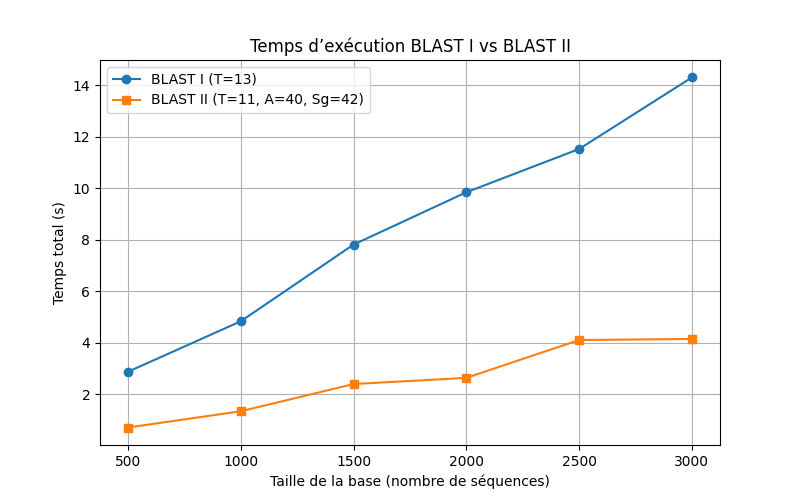
\includegraphics[width=0.45\textwidth]{test_temps.png}
    \caption{Temps total d’exécution en fonction de la taille de la base
    pour BLAST I et BLAST II.}
    \label{fig:time_vs_dbsize}
\end{figure}

\section{Discussion}

\subsection{Comparaison avec les articles initiaux}
Nos résultats expérimentaux confirment globalement les tendances décrites dans les articles fondateurs de BLAST et de gapped blast.\\
Tout d’abord, nous avons reproduit la forte proportion de temps consacrée à l’extension dans BLASTI (plus de $90\%$), contre une répartition beaucoup plus équilibrée dans BLAST II (\approx $60-70\%$ extension gappée et $30-40\%$ détection de double-hits).\\
Ce profil correspond à celui rapporté dans la littérature.\\

De plus, nous avons observé le même renversement dans la courbe du nombre d’alignements acceptés : BLAST I est plus sensible pour des seuils faibles mais génère beaucoup de bruit, tandis que BLAST II devient supérieur lorsque l’on impose des seuils plus stricts, grâce à l’extension gappée et à un $x\_{drop}$ plus permissif.\\
Ce comportement correspond aux figures de sensibilité et de vitesse publiées en 1997, où les auteurs concluent que le gapped BLAST est à la fois trois fois plus rapide et plus robust} que la version originale.

\subsection{Limites}
Nos implémentations restent toutefois limitées par plusieurs aspects.\\
Premièrement, les expériences ont été menées sur des bases aléatoires de taille modeste, ce qui ne reflète pas totalement la complexité des bases biologiques réelles.\\
Deuxièmement, nous n’avons pas encore intégré l’évaluation statistique complète via les paramètres de Karlin–Altschul ($\lambda$, $K$, $E$-value), ce qui nous empêche de déterminer si un alignement obtenu présente un intérêt biologique, ou si c'est seulement le bruit qui parle.\\
Enfin, de nombreuses manières d'accélerer les algorithmes restent encore à implémenter (parallélisme, structure de données plus efficaces, algorithmes de programmation dynamique).

\subsection{Améliorations}
Plusieurs pistes d’amélioration sont envisageables.
Tout d'abord, l’utilisation de données réelles (familles de protéines connues) permettrait d’évaluer le nombre d’alignements significatifs manqués par BLAST I et BLAST II par rapport à un algorithme optimal (comme Smith–Waterman).\\
L’ajout d’une estimation statistique rigoureuse des $E$-values permettrait également de rendre les résultats directement exploitables dans un contexte biologique.\\
Sur le plan algorithmique, l’introduction de structures compressées pour stocker la base ou l’intégration d'algorithmes d’alignement optimisées (via  parasail par exemple) permettrait d’atteindre des performances proches des implémentations publiques de BLAST.\\
Enfin, un prolongement naturel de ce travail serait l’exploration de PSI-BLAST, qui améliore considérablement la sensibilité par itérations successives tout en conservant une vitesse d’exécution proche de BLAST II.

\end{document}
